\chapter*{JANUS INTERLUDE}\label{JANUS INTERLUDE}
\addcontentsline{toc}{chapter}  {JANUS INTERLUDE}
\markboth{JANUS INTERLUDE}{}

\begin{center}
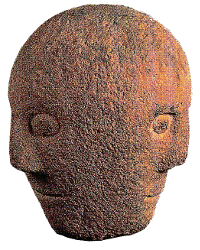
\includegraphics[max width=\textwidth]{janus_rock_200x250}
\end{center}

Janus has rightly been adopted as the god of whole systems. He can look forwards and backwards simultaneously, and thus symbolises the closed loop at the heart of all cybernetic systems.

This Janus interlude is included at roughly the halfway point in the book to provide the reader with a perspective on where he's been and where he's going.

Looking back ...

Having completed the Preliminary Diagnosis, you should by now have a thorough feel for the form of the model.

\begin{itemize}
  \item The separation of Operation, Metasystem and Environment

  \item The small VSMs nested recursively within the Operation

  \item The four Metasystemic functions

\end{itemize}

If you have been drawing the pictures, you should by now have a number of large VSM sketches, showing the five systems and the bits of your organisation which do those jobs, and you will probably have had a Eureka! or two, as the VSM version of organisational reality unfolded.

Looking forward ...

So where do we go from here?

I admit that my first few attempts at using the VSM finished here, despite a few nagging doubts about Beer's Laws and Axioms, which didn't really seem to fit in anywhere.

After much further reading and discussion it became clear that the job had only been half-completed. YES, I had identified the five systems at various levels of recursion, but NO, the diagnosis was by no means complete.

Consider now, the Viable Vehicle Model, or VVM, a guaranteed fool-proof methodology for the diagnosis and design of any vehicle, regardless of size or the terrain on which it must travel, based cybernetically on the invariances in vehicular functioning.

The VVM is composed of 5 systems:

\begin{enumerate}
  \item Some means of propulsion
  \item Some means of steering
  \item Something to carry the load
  \item A method of reducing friction
  \item Some way of stopping
\end{enumerate}

Imagine you have completed the Preliminary Diagnosis of your Vehicle-in-Focus (or VIF) that you have successfully identified the five systems, and drawn a big diagram to illustrate their basic relationships.

So what now? Is the VVM diagnosis complete? Again you may have a few nagging doubts about the VIF as a whole. For example, you may be concerned that your design of your Propulsion System One (in this case a very substantial rubber band) is not quite up to the job of moving the Vehicle with the 400 tonne loads you envisage. Similarly System 5 (a large rock on the end of a rope) has been clearly identified as a fine example of the stopping function, but as the vehicle is intended to transport steel in Alaska (and thus has System 4 consisting of skis) doesn't look too reliable.

The overriding questions begin to emerge: Do the parts add up to a workable whole? Are the parts balanced to complement one another?

VVM practitioners will know that the workings of the whole is a very different thing from the workings of the parts. In some cases overall improvements in efficiency may be the result of actually decreasing the capabilities of one sub-unit.

So, if the vehicle is on wheels, are the brakes and engine designed to match the weight and speeds for which the vehicle is designed? If the vehicle is a hovercraft, the engine could be smaller as friction is minimal, but this may present more problems for the design of the stopping and steering systems.

\begin{center}
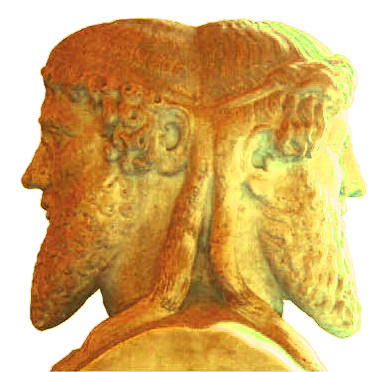
\includegraphics[max width=\textwidth]{Janus_383x372}
\end{center}

The conclusion is:

\begin{itemize}
  \item The design of the whole system must be considered.

  \item Just because the parts are there, there is no reason why they should work together to produce an effective whole.

\end{itemize}

And exactly the same is true of the VSM.

In my initial studies, I had not looked at the way the parts interact, how they work together to generate a well-designed whole, how the capabilities of the regulatory systems balance the problems they are dealing with.

Everything which follows is about balance.

The essence is well-balanced, whole-system design.

This is where the forward-looking head of Janus is looking.